\documentclass[11pt, oneside]{article} 
\usepackage{geometry}
\geometry{letterpaper} 
\usepackage{graphicx}
	
\usepackage{amssymb}
\usepackage{amsmath}
\usepackage{parskip}
\usepackage{color}
\usepackage{hyperref}

\graphicspath{{/Users/telliott_admin/Tex/png/}}
% \begin{center} 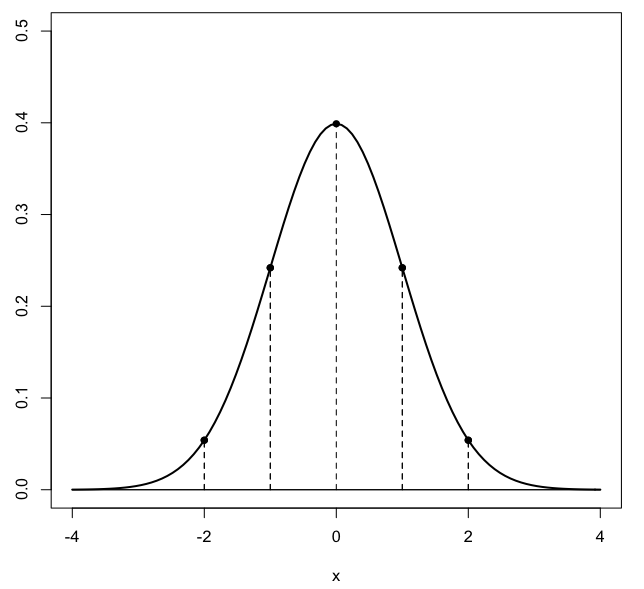
\includegraphics [scale=0.4] {gauss3.png} \end{center}

\title{Series convergence}
\date{}

\begin{document}
\maketitle
\Large

\subsection*{Tests for convergence}
Series like the Taylor series can be very helpful in approximating a function.  Here we review some common tests to see whether the sum of an infinite series converges to a finite limit, or instead diverges.

Start with the geometric series
\[ \sum_{k=0}^{\infty} x^k \]
Suppose we compute the sum of a number of terms $n$
\[ s_n = x^0 + x^1 + x^2 + \dots + x^n \]
Since this is a finite series, the sum exists so
\[ x s_n = x^1 + x^2 + \dots + x^{n+1} \]

Then
\[ s_n - x s_n = (1-x) s_n = 1 - x^{n+1} \]
\[ s_n = \frac{1}{1-x} - \frac{x^{n+1}}{1-x}, \ \ \ x \ne 1 \]

Clearly, if $x>1$ then $x^{n+1} \rightarrow \infty$ as $n$ gets large, and this is true even if $x = 1$.  If $x<-1$ then the second term alternates in sign and its absolute value gets very large as $n$ gets large.  

Only for $|x| < 1$, as $n \rightarrow \infty$, the second term vanishes and we have
\[ s_n = \frac{1}{1-x} \]
For example,
\[ \sum_{k=0}^{\infty} (\frac{1}{2})^k = \frac{1}{1-1/2} = 2 \]
\[ \sum_{k=0}^{\infty} (\frac{1}{3})^k = \frac{1}{1-1/3} = \frac{3}{2} \]
and so on.

A second famous series is the harmonic series
\[ \sum_{k=0}^{\infty} \frac{1}{k^p} \]
especially with $p=1$
\[ \sum_{k=0}^{\infty} \frac{1}{k} = 1 + \frac{1}{2} + \frac{1}{3} + \dots \]
This series diverges.  

One proof is the following.  Assume that the series converges.  Then its sum has a limit which we can call $L$.
\[ L = 1 + \frac{1}{2} + \frac{1}{3} + \frac{1}{4} +  \frac{1}{5} +  \frac{1}{6} \dots \]
\[ > \frac{1}{2} + \frac{1}{2} + \frac{1}{4} + \frac{1}{4} +  \frac{1}{6} +  \frac{1}{6}  \dots \]
\[ = 1 + \frac{1}{2} + \frac{1}{3} \dots \]
\[ = L \]
a contradiction.  Therefore, the harmonic series diverges.

Let us look at some tests of convergence.

\subsection*{Divergence test}
The first test requires that the limit of the individual terms $a_k$ must tend to zero
\[ \lim_{k \rightarrow \infty} a_k = 0 \]
if not, then the sum diverges.  For example,
\[ \frac{1}{2} + \frac{2}{3} + \frac{3}{4} + \frac{4}{5} + \dots \]
This clearly diverges, since
\[ \lim_{k \rightarrow \infty} a_k = 1 \]
Or
\[ \lim_{k \rightarrow \infty} \frac{k}{2k + 1}, \ \ \ k \in \{1,2,\dots\} \]
\[ = \lim_{k \rightarrow \infty} \frac{1}{2 + 1/k} = \frac{1}{2} \ne 0 \]
Another example is the harmonic series
\[ \lim_{k \rightarrow \infty} \frac{1}{k} = 0, \ \ \ k \in \{1,2,\dots\} \]
Despite passing this limit test, the harmonic series diverges.  Thus, a pass is necessary but not sufficient.

\subsection*{Integral test}
The integral test says that a (well-behaved) function $f(x)$
\[ \int_1^{\infty} f(x) \ dx \]
converges $\iff$
\[ \sum_{k=1}^{\infty} f(k) \]
also converges.  The function must be continuous and integrable, etc.

Let's apply this test to the harmonic series
\[ \sum_{k=0}^{\infty} \frac{1}{k} \]
We have
\[ \int_1^{\infty} \frac{1}{x} \ dx = \ln |x| \ \bigg |_1^{\infty} \]
but the upper bound has the limit
\[ \lim_{k \rightarrow \infty} \ln |k| = \infty \]

In general, for
\[ \sum_{k=0}^{\infty} \frac{1}{k^p} \]
if $p>1$, the sum converges, but not otherwise:
\[ \int_1^{\infty} x^{-p} \ dx = \frac{1}{1-p}x^{1-p} \ \bigg |_1^{\infty} \]
For $p>1$
\[ \lim_{x \rightarrow \infty} x^{1-p} = 0 \]
On the other hand
\[ \int_1^{\infty} \frac{1}{n^2} \ dn = - \frac{1}{n} \ \bigg |_1^{\infty} = 0 - - 1 = 1 \]
so the $\sum 1/n^2$ converges.

\subsection*{Comparison test}
If we compare a series and a convergent series and the test series is smaller term-by-term, then it also converges.  Similarly, if a series is larger than a divergent series when compared term-by-term, it also diverges.  Any finite number of terms from the beginning of a series may be disregarded before starting the comparison.

Since
\[ \sum_{k=0}^{\infty} \frac{1}{k^2} \] 
converges, so does
\[ \sum_{k=0}^{\infty} \frac{1}{k^2 + 10} \] 
And since
\[ \sum_{k=0}^{\infty} \frac{1}{k} \] 
diverges, so does
\[ \sum_{k=0}^{\infty} \frac{1}{\ln|k+1|} \] 
since for $k>2$
\[ \ln|k+1| < k \]
 so
\[ \frac{1}{\ln|k+1|} > \frac{1}{k} \]

\subsection*{Ratio test}
Consider
\[ \sum_{k=0}^{\infty} a_k, \ \ \ a_k > 0 \] 
\[ \lim_{k \rightarrow \infty} \frac{a_{k+1}}{a_k} = L \]

\begin{displaymath}
   \left\{
     \begin{array}{lr}
       L < 1 & : \text{converges} \\
       L > 1 & : \text{diverges} \\
	   L = 1 & : \text{inconclusive}
     \end{array}
   \right.
\end{displaymath} 
As an example
\[ \sum_{k=0}^{\infty} \frac{1}{k!} \]
Check
\[ \lim_{k \rightarrow \infty} \frac{1/(k+1)!}{1/k!} = \frac{1}{k+1} < 0 \]
This one is also easily checked by the comparison test since
\[ k! > k^2, \ \ \ k > 3 \]
Since $1/k^2$ converges, so does $1/k!$.

Or
\[ 1 + \frac{1}{2} + \frac{1}{3} + \frac{1}{4} + \dots \]
\[ \lim_{k \rightarrow \infty} \frac{1/n+1}{1/n} = \frac{n}{n+1} = 1 \]
so the test is inconclusive.

\subsection*{a bit more}
In the previous chapter, we looked at Taylor series and showed that
\[ \ln 2 = 1 - \frac{1}{2} + \frac{1}{3} - \frac{1}{4} + \frac{1}{5} - \cdots \]

Actually, this series is really interesting from the point of view of convergence.  An infinite series is convergent if all of the terms add up to something finite, like $\ln 2$.

In this case, the terms alternate sign, which makes me wonder.  We have the positive terms
\[ 1 + \frac{1}{3} + \frac{1}{5} + \frac{1}{7} + \frac{1}{9} +  \dots \]
The two terms
\[  \frac{1}{5} + \frac{1}{7} = \frac{12}{35} = 0.343 > \frac{1}{3} \]
The next four terms
\[ \frac{1}{9} + \frac{1}{11} + \frac{1}{13} + \frac{1}{15}  \]
\[ =  \frac{715}{6435} + \frac{585}{6435} + \frac{495}{6435} + \frac{429}{6435} = \frac{2224}{6435} \]
\[ = 0.346 > \frac{1}{3} \]

Notice that the decimal sum is increasing.

This is sorta like the harmonic series.  It diverges to $+ \infty$.

The negative terms are

\[ - \frac{1}{2} - \frac{1}{4} - \frac{1}{6} - \frac{1}{8} + \cdots \]
\[ = (-\frac{1}{2}) \cdot (1 + \frac{1}{2} + \frac{1}{3} + \frac{1}{4} + \dots \]
which \emph{is} the harmonic series.  It diverges to $- \infty$.

So two series which separately diverge to $+ \infty$ and  $- \infty$ add to something finite!

Another amusing rearrangement of the $\ln 2$ series (Acheson) is:
\[ 1 - \frac{1}{2} + \frac{1}{3} - \frac{1}{4} + \frac{1}{5} - \frac{1}{7} + \frac{1}{8} +  \cdots \]
\[ = (1 - \frac{1}{2}) - \frac{1}{4} + (\frac{1}{3} - \frac{1}{6}) - \frac{1}{8} + (\frac{1}{5} - \frac{1}{10}) - \frac{1}{12} + \dots \]
\[ = \frac{1}{2} - \frac{1}{4} + \frac{1}{6} - \frac{1}{8} + \frac{1}{10} - \frac{1}{12} + \dots \]
\[ = \frac{1}{2} (1 - \frac{1}{2} + \frac{1}{3} - \frac{1}{4} + \frac{1}{5} - \frac{1}{6} + \dots) \]

How can the series be equal to one-half of itself?

These groupings of terms with alternating signs are illegal.  They do not yield correct values for the sum.  However, an adjacent grouping does work, namely:

\[ (1 - \frac{1}{2}) + (\frac{1}{3} - \frac{1}{4}) + (\frac{1}{5} - \frac{1}{6}) + (\frac{1}{7} - \frac{1}{8}) +   \cdots \]
\[ = \frac{1}{2} + \frac{1}{12} + \frac{1}{30} + \frac{1}{56} + \dots \]

which, as you can see, converges rather slowly.

\end{document}  